

\section{Introduction}





Although large language models (\llms) can generate coherent outputs, they often fall short in addressing intricate requirements. This mostly includes tasks
with multifaceted objectives, 
such as dialogue response generation, or tasks with hard-to-define goals, such as enhancing program readability. 
In these scenarios, modern \llms may produce an intelligible initial output, yet may benefit from further iterative refinement---i.e., iteratively mapping a candidate output to an improved one---to ensure that 
the desired quality is achieved. 
Iterative refinement typically involves training a refinement model that relies on domain-specific data (e.g., \citet{reid2022learning,timoschick2022PEER,Welleck2022SelfCorrect}).
Other approaches that rely on external supervision or reward models require large training sets or expensive human annotations ~\citep{madaan2021graphcorr, Ouyang2022TrainingLM}, which may not always be feasible to obtain. %
These limitations underscore the need for an effective refinement approach
that can be applied to various tasks without requiring extensive supervision.








Iterative \emph{self}-refinement is a fundamental characteristic of human problem-solving \citep{simon1966complexity,flower1981cognitive,amabile_theoretical_1983}. Iterative self-refinement is a process that involves creating an initial draft and subsequently refining it based on self-provided feedback.
For example, when drafting an email to request a document from a colleague, an individual may initially write a direct request such as ``\textit{Send me the data ASAP}''.
Upon reflection, however, the writer recognizes the potential impoliteness of the phrasing and revises it to ``\textit{Hi Ashley, could you please send me the data at your earliest convenience?}". 
When writing code, a programmer may implement an initial ``quick and dirty'' implementation, and then, upon reflection, refactor their code to a solution that is more efficient and readable.
In this paper, we demonstrate that LLMs can provide 
iterative self-refinement without additional training, leading to higher-quality outputs on a wide range of tasks.

We present \ours: an iterative self-refinement algorithm that alternates %
between two generative steps--\fbmod and \itermod. These steps work in tandem to generate high-quality outputs.
Given an initial output generated by a model $\mathcal{M}$, 
we pass it back to the same model $\mathcal{M}$ to get \emph{feedback}.
Then, the feedback 
is passed back to the same model to \textit{refine} the previously-generated draft. %
This process is repeated either for a specified number of iterations or until $\mathcal{M}$ determines that no further refinement is necessary. We use few-shot prompting~\citep{brown2020language} to guide $\mathcal{M}$ to both generate feedback and incorporate the feedback into an improved draft.
\Cref{fig:mainfig} illustrates the high-level idea, that \emph{\ours uses the same underlying language model to  generate feedback and refine its outputs}. %



\begin{figure*}[t]
    \centering
    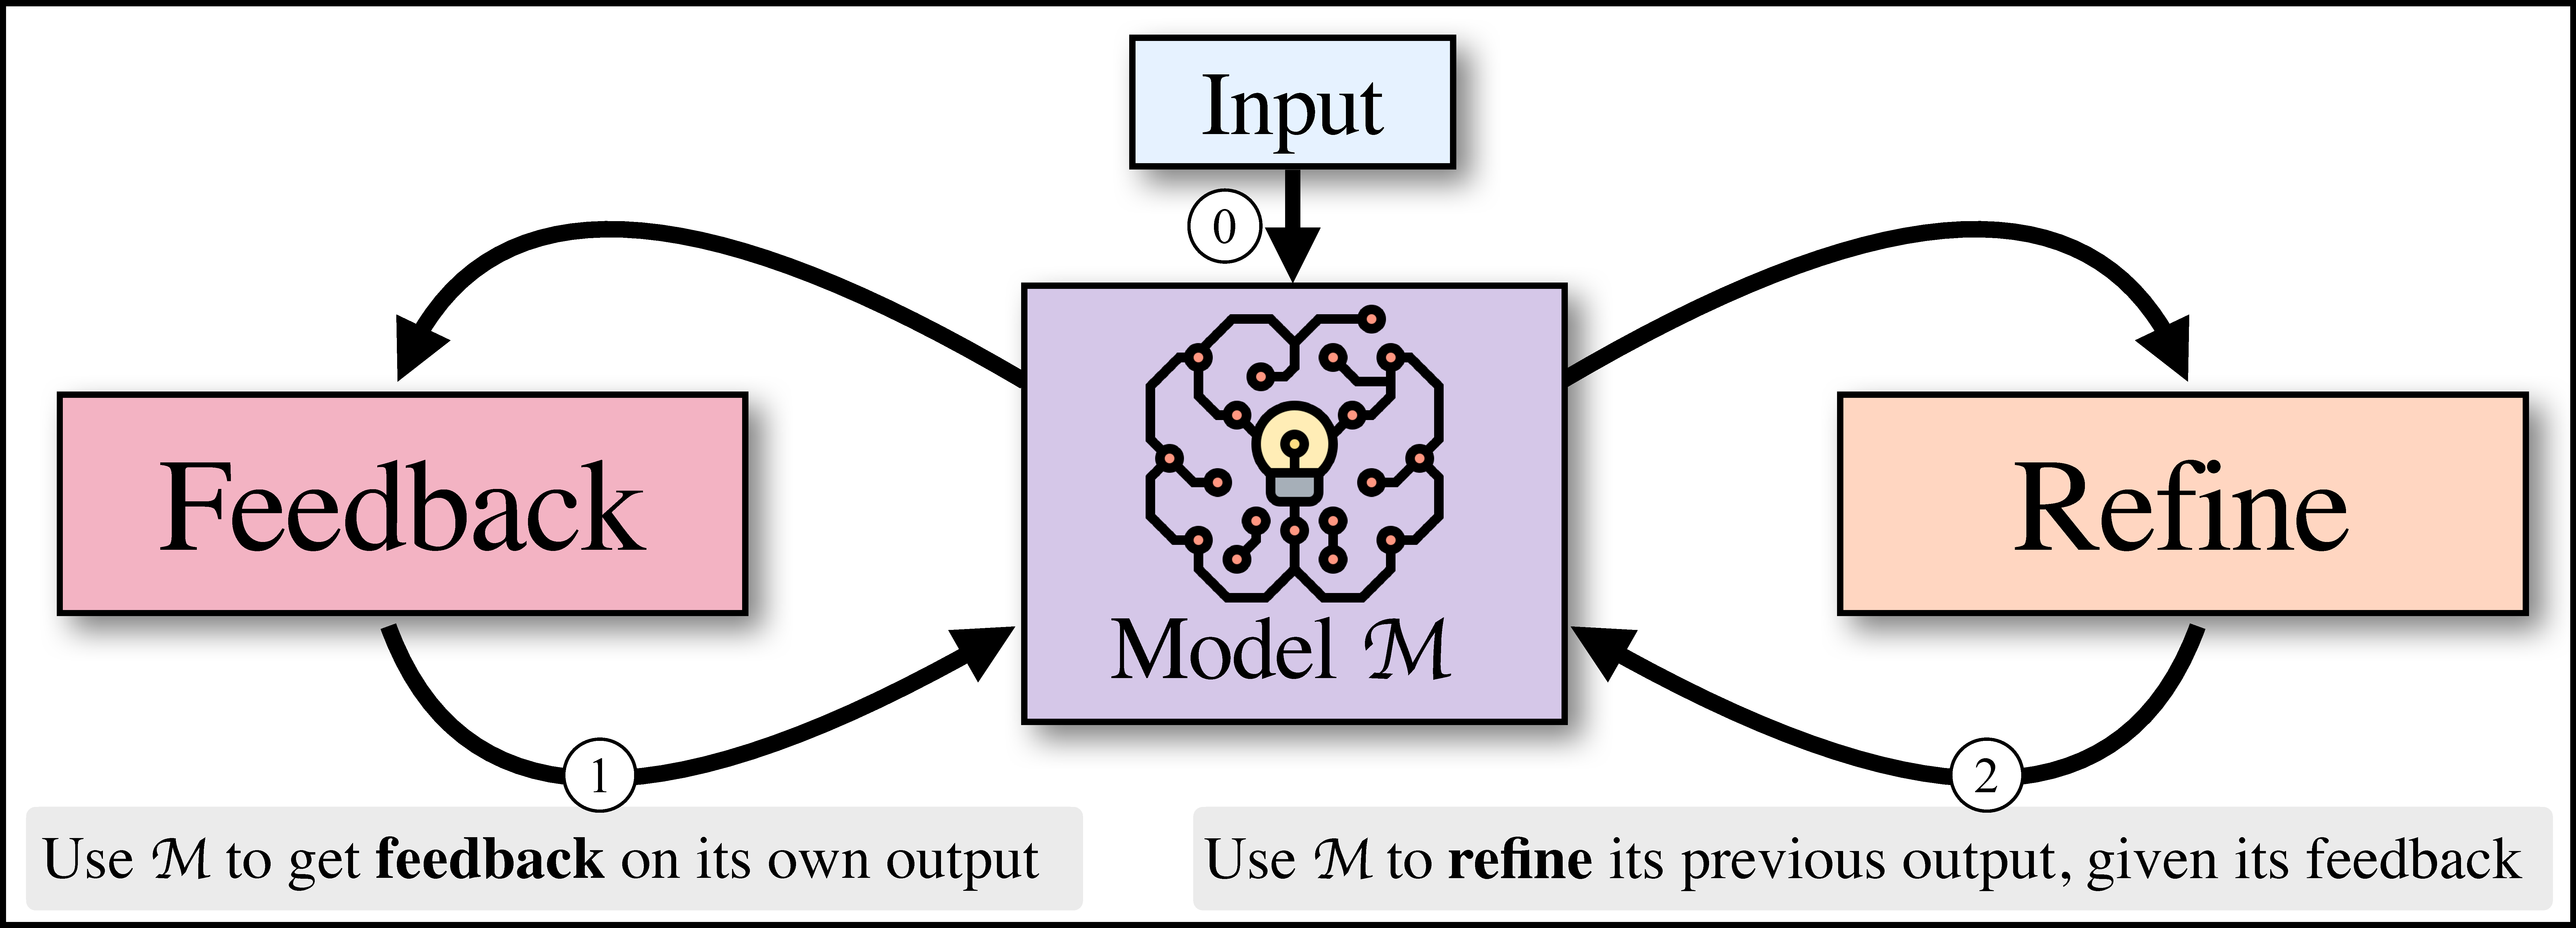
\includegraphics[width=0.9\textwidth]{figures/autofb_figv3.pdf}
    \caption{
    Given an input (\circnum{0}), \ours starts by generating an output and passing it back to the same model $\mathcal{M}$ to get feedback (\circnum{1}). The feedback is passed back to $\mathcal{M}$, which refines the previously generated output  (\circnum{2}). Steps (\circnum{1}) and (\circnum{2}) iterate until a stopping condition is met. \ours  is instantiated with a language model such as \gptt and does not involve  human assistance.
    }
    \label{fig:mainfig}
\end{figure*}


We evaluate \ours on \numtasks generation tasks that span diverse domains, including natural language and source-code generation.
We show that \ours outperforms direct generation from strong \llms like \gptt \citep[\texttt{text-davinci-003} and \texttt{gpt-3.5-turbo}; ][]{openai_model_index,Ouyang2022TrainingLM} and \gptf \citep{openai2023gpt4} 
by 5-40\% absolute improvement.
In code-generation tasks, \ours improves the initial generation by up to absolute 13\% when applied to strong code models such as Codex \citep[\texttt{code-davinci-002}; ][]{codex}. We release all of our code, which is easily extensible to other LLMs.
In essence, our results show that even when an \llm cannot generate an optimal output on its first try, the \llm can often provide useful feedback and improve its own output accordingly.
In turn, \ours provides an effective way %
to obtain better outputs from a single model without any additional training, via iterative (self-)feedback and refinement. 










